%% LaTeX-Beamer template for KIT design
%% by Erik Burger, Christian Hammer
%% title picture by Klaus Krogmann
%%
%% version 2.1
%%
%% mostly compatible to KIT corporate design v2.0
%% http://intranet.kit.edu/gestaltungsrichtlinien.php
%%
%% Problems, bugs and comments to
%% burger@kit.edu

\documentclass[18pt]{beamer}
%% SLIDE FORMAT
\usepackage[utf8]{inputenc}
\usepackage{algpseudocode}
\usepackage{amssymb}
% use 'beamerthemekit' for standard 4:3 ratio
% for widescreen slides (16:9), use 'beamerthemekitwide'

\usepackage{templates/beamerthemekit}
% \usepackage{templates/beamerthemekitwide}


%% TikZ INTEGRATION

% use these packages for PCM symbols and UML classes
% \usepackage{templates/tikzkit}
% \usepackage{templates/tikzuml}

% the presentation starts here

\title[Programmieren Tutorium]{8. Programmieren Tutorium:\texorpdfstring{\\}{}Der Vererbung zweiter Teil}
\subtitle{noch mehr was dazugehört}
\author{Konstantin Zangerle \texorpdfstring{\\}{} info@konstantinzangerle.de}
\date{16. Dezember}
\institute{Chair for Software Design and Quality}

\usepackage{listings}
\usepackage{color}

\definecolor{mygreen}{rgb}{0,0.6,0}
\definecolor{mygray}{rgb}{0.5,0.5,0.5}
\definecolor{mymauve}{rgb}{0.58,0,0.82}

\lstset{ %
  backgroundcolor=\color{white},   % choose the background color
  basicstyle=\footnotesize,        % size of fonts used for the code
  breaklines=true,                 % automatic line breaking only at whitespace
  captionpos=b,                    % sets the caption-position to bottom
  commentstyle=\color{mygreen},    % comment style
  escapeinside={\%*}{*)},          % if you want to add LaTeX within your code
  keywordstyle=\color{blue},       % keyword style
  stringstyle=\color{mymauve},     % string literal style
  showstringspaces=false,
  language=Java
}
\beamersetuncovermixins{\opaqueness<1>{0}}{\opaqueness<2->{0}} %Dont show things after pause 
% Bibliography

\usepackage[citestyle=authoryear,bibstyle=numeric,hyperref,backend=biber]{biblatex}
\addbibresource{templates/example.bib}
\bibhang1em


\begin{document}
% change the following line to "ngerman" for German style date and logos
\selectlanguage{ngerman}

%title page
\begin{frame}
\titlepage
\end{frame}

%table of contents
\begin{frame}{Gliederung}
\tableofcontents
\end{frame}
\section{ToDo-Liste}
\begin{frame}[fragile]{ToDo-Liste}
\begin{itemize}
 \item Vererbung \checkmark
 \item Dynamische Bindung
 \item Überschreibung von Attributen und Methoden \checkmark
 \item Konstruktoren mit \verb|super| \checkmark
 \item Typumwandlungen 
 \item Klasse \verb|Object| und Java-Klassenhierarchie
 \item Abstrakte Klassen
 \item Inhaltliche Gleichheit
 \item \verb|final|
 \item Javadoc \checkmark
 \item Verkette Listen und Iteratoren
 \item Queue, Stack, Priority Queue
 \item Schnittstellen \checkmark
 \item Generische Klassen und Schnittstellen \checkmark
  \item \verb|instanceof|
\end{itemize}
\end{frame}

\begin{frame}[fragile]{Heute}
\begin{itemize}
 \item Dynamische Bindung
 \item Typumwandlungen
 \item Klasse \verb|Object| und Java-Klassenhierarchie
 \item Abstrakte Klassen
 \item Inhaltliche Gleichheit
 \item \verb|final|
 \item Verkettete Listen und Iteratoren
 \item Queue, Stack, Priority Queue
 \item \verb|instanceof|
\end{itemize}
\end{frame}

\section{Organisatorisches}
\begin{frame}{Kein Tut am 23.12}
 \large FROHE WEIHNACHTEN!!!
 
 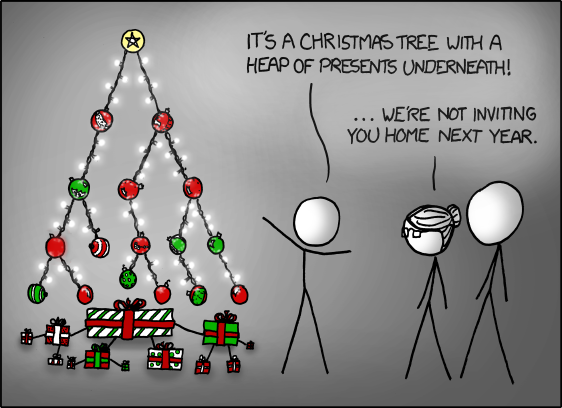
\includegraphics[scale=0.5]{08_tree}
 \tiny: xkcd.com/835/
\end{frame}


\section{Stoff}
\subsection{Dynamische Bindung}
\begin{frame}[fragile]{Dynamische Bindung}

 \begin{lstlisting}
public class GameObject {
  public String name;
  @Override public String toString()   {
    return String.format( "GameObject[name=%s]", name );
  }
}
public class Room extends GameObject {
  public int size;
  @Override public String toString()  {
    return String.format( "Room[name=%s, size=%d]", name, size );
  }
} \end{lstlisting}

\end{frame}

\begin{frame}[fragile]{Welche Ausgabe erwartet ihr?}
 \begin{lstlisting}
Room rr = new Room();
rr.name = "Affenhausen";
rr.size = 7349944;
System.out.println( rr.toString() );
GameObject rg = new Room();
rg.name = "Affenhausen";
System.out.println( rg.toString() );
Object ro = new Room();
System.out.println( ro.toString() );
 \end{lstlisting}
 \pause
 \begin{lstlisting}
---
Room[name=Affenhausen, size=7349944]
Room[name=Affenhausen, size=0]
Room[name=null, size=0]
\end{lstlisting}

\end{frame}

\subsection{Typumwandlung}
\begin{frame}[fragile]{Typumwandlungen}
 Gehen wir einmal die Tests durch:
 \verb|http://www.java-tutorial.org/typecasting.html|
\end{frame}

\begin{frame}{Widening and Narrowing Conversions}
 \includegraphics{08_narrowing}
 \includegraphics{08_widening}
\end{frame}

\subsection{Java-Object}
\begin{frame}{Java: Object}
  \small
 Jedes Objekt hat folgende Methoden:
 \begin{itemize}
  \item clone()
  \item equals(Object obj)
  \item finalize()
  \item getClass()
  \item hashCode()
  \item notify()
  \item notifyAll()
  \item toString()
  \item wait()
  \item wait(long timeout)
  \item wait(long timeout, int nanos)
 \end{itemize} \pause
 Aber warum? \pause \\
 \large Antwort: Vererbung
 

\end{frame}
\begin{frame}{Java-Klassenhierarchie}
 
\end{frame}

\begin{frame}[fragile]{Abstrakte Klassen}
 Abstrakte Klassen sind Klassen, die nicht direkt instanziert werden können.
 \begin{lstlisting}
    public abstract class AbstracterSchinken {
      public String name;
    }
 \end{lstlisting} \pause
 Natürlich gilt das auch für Methoden
 \begin{lstlisting}
    public abstract class AbstrakterSchinken {
      public abstract void Abschneiden();
    }
 \end{lstlisting} \pause
Was ist der Unterschied einer abstrakten Klasse zu ``Interfaces``?
\end{frame}

\begin{frame}[fragile]{Inhaltliche Gleichheit}
 Java erlaubt es zunächst auf Identität zu überprüfen.
 Mittels \verb|==|
 \begin{itemize}
  \item Das funktioniert nicht bei Strings.
  \item Zumindest meistens.
  \item Siehe letztes Übungsblatt.
 \end{itemize}
\end{frame}
\begin{frame}[fragile]{Prüfen auf ''Inhaltliche Gleichheit''}
 Mittels überschreiben der \verb|equals|-Methode. Alles klar? \pause
 Was gibt es zu beachten?:
 Equals muss erfüllen
 \begin{enumerate}
  \item Reflexiv
  \item Symmetrisch
  \item Transitiv
  \item Konsistenz
  \item für x nicht null gibt x.equals(null) false
 \end{enumerate}
\end{frame}

\begin{frame}[fragile]{Beispiel}
 \begin{lstlisting}
  public boolean equals(Object other) {
   if (this == other)
      return true;
   if (other == null)
      return false;
   if (other.getClass() != getClass())
      return false;

   if (!(s.equals(((MyClass)other).s)))
      return false;
   if (i != ((MyClass)other).i)
      return false;
   ...
   return true;
   } 
 \end{lstlisting}
\end{frame}

\begin{frame}{Final}
„Bis hierher darfst du und nicht weiter, hier muss sich legen deiner Wogen Stolz“. (Ijob 38,11)
  \pause
  
  \begin{itemize}
   \item Klassen: Kann nicht abgeleitet werden
   \item Methoden: Kann nicht überschrieben/versteckt werden
   \item Variablen: Kann nur einmal initialisiert werden, jede Änderung erzeugt einen Fehler
  \end{itemize}
\end{frame}

\begin{frame}{Verkettete Listen und Iteratoren}
 siehe IteratorTest.java
\end{frame}

\

\begin{frame}[fragile]{Was noch?}
\begin{itemize}
 \item Dynamische Bindung \checkmark
 \item Typumwandlungen \checkmark
 \item Klasse \verb|Object| und Java-Klassenhierarchie \checkmark
 \item Abstrakte Klassen \checkmark
 \item Inhaltliche Gleichheit \checkmark
 \item \verb|final| \checkmark
 \item Verkettete Listen und Iteratoren \checkmark
 \item Queue, Stack, Priority Queue
 \item \verb|instanceof|
\end{itemize}
\end{frame}

\begin{frame}{Queue, Stack, Priority Queue}
 
\end{frame}

\begin{frame}{instanceof}
 
\end{frame}









%%%% Ab hier muss nur noch das Bild gewechselt werden...
\section{Fragen zum Übungsblatt?}
\begin{frame}{Fragen?}
\end{frame}



%Lacher zum Schluss
\begin{frame}{}
 \includegraphics[scale=0.4]{08_questions}
 
 \tiny{Quelle: xkcd.com}
\end{frame}


\end{document}
%%%%%%%%%%%%%%%%%%%%%%%%%
%Bausteine
%nice to have code
%%%%%%%%%%%%%%%%%%%%%%%%%%


%%%%% Bausteine Folie mit Java-Code
%\begin{frame}[fragile]{bla}
%\begin{exampleblock}{bla}
%\begin{lstlisting}[language=java]
%\end{lstlisting}
%\end{exampleblock}
%\end{frame}
